\documentclass[10pt]{article}\usepackage[margin=.55in]{geometry}\usepackage[T1]{fontenc}\usepackage{graphicx}\setlength{\parindent}{0pt}\setlength{\parskip}{4pt}\sloppy\begin{document}{\large Supervisor v3 and retained-image qualification draft}\par The successor supervisor fixes the observed reconciliation error by requesting losetup list mode explicitly. A strict parser accepts only a JSON object with exactly one loopdevices field containing an empty list. Empty bytes, malformed shapes, duplicate keys and attached devices fail closed. All 36 producer software controls passed: the 29 retained controls and seven focused parser/reconciliation controls.\par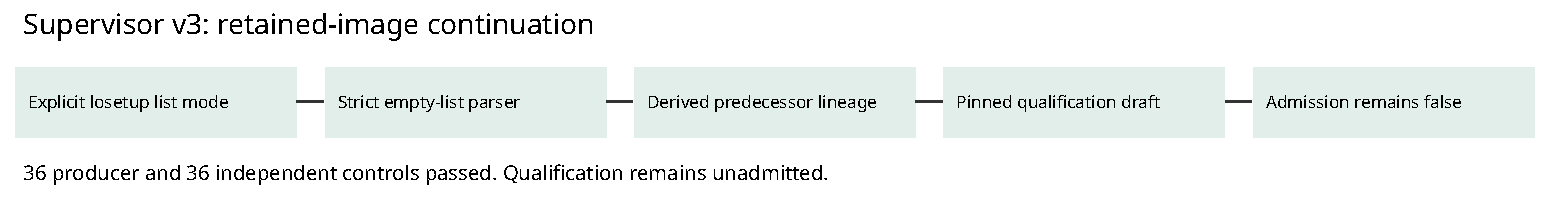
\includegraphics[width=.96\linewidth]{diagram.pdf}\par Retained predecessor. A separate derived receipt combines the exact successful worker result with the independently reviewed read-only disposition and its successful execution receipt. It records the original launcher failure and hashes, the reconciliation source/review/publication, and that the disk hash is inherited from the worker under unchanged custody. The original failed receipt and v2 supervisor are preserved. The derived assembled\_stopped status is explicitly an observation-derived compatibility receipt, not a rewritten original launcher result.

Qualification draft. The existing fresh qualification owner is bound to the retained image, private disk, reviewed qualifier source closure, source manifest, fixtures, and the held-release gate with 45 parser and 154 helper controls. A new gate copy has mode 0555 and one hard link; its digest matches the retained candidate. No gate binary was executed. Expected build metadata is reused from its pinned prior evidence and remains subject to actual image readback during qualification.

Resource envelope. The draft retains one 300-second qualification phase, 2 CPU quota, 2 GiB RAM, zero swap, 256 tasks and the existing 4 GiB private disk, with a 30-second reserve and 5-second stop limit. It does not rebuild or reload the retained image. Both admission flags remain false. A prospective independent qualification review, exact review-input binding and remaining campaign accounting are still needed before execution.

Validation. One producer software invocation used a 60-second outer timeout plus 5-second kill reserve, 512 MiB address space and 55-second child timeout. Tests used mocks and local temporary files. Independent review replayed all 36 tests and accepted the source delta; the derived receipt also binds the actual disposition postreview. No daemon, mount, service launch, qualification or scientific trajectory was run by this packet.
\end{document}